\documentclass[12pt,twoside, a4paper, twocolumn]{article}
\usepackage[utf8]{inputenc}
\usepackage[brazil]{babel}
\usepackage[margin = 0.5in]{geometry}
\usepackage{amsmath}
\usepackage{amsthm}
\usepackage{amssymb}
\usepackage{amsthm}
\usepackage{setspace}
\usepackage[americanvoltages,fulldiodes,siunitx]{circuitikz}
\usepackage{lipsum}
\usepackage{pgfplots}
\usepackage{ifthen}
\usepackage{adjustbox}
\usepackage[section]{placeins}
\usepackage{hyperref}
\usepackage{graphicx}
\usepackage{amsmath}
\usepackage{amsthm}
\usepackage{amssymb}
\usepackage{amsthm}
\usepackage{setspace}
\usepackage[americanvoltages,fulldiodes,siunitx]{circuitikz}
\usepackage{lipsum}
\usepackage{pgfplots}
\usepackage{ifthen}
\usepackage{adjustbox}
\usepackage[section]{placeins}
\usepackage{hyperref}
\usepackage{graphicx}
\usepackage{adjustbox}
\usepackage{indentfirst}








\pgfplotsset{compat=newest}
\graphicspath{ {./images/} }
%  #1 color - optional #2 x_0 #3 y_0 #4 x_f #5 y_f #6 name - optional  #7 true if adding lines to axis
\newcommand{\drawvector} [9] [color=cyan] {
\draw[line width=1.5pt,#1,-stealth](axis cs: #2, #3)--(axis cs: #4, #5) node[anchor=south west]{$#6$};
\ifthenelse{\equal{#7}{true}}{
\draw[line width=1pt,#1, dashed](axis cs: #4, #5)--(axis cs: #4, 0) node[anchor= north west]{$#8$};
\draw[line width=1pt,#1, dashed](axis cs: #4, #5)--(axis cs: 0, #5) node[anchor=south east]{$#9$};
}
{}
}
\newcommand\deriv[2]{\frac{\mathrm d #1}{\mathrm d #2}}
\title{Primeiro Relatório de Eletronica Digital}
\author{ Bruno Franca - emailaqui
\\ Gabriela Leite - emailaqui
\\ Henrique da Silva - henrique.pedro@ufpe.br
\\ Pedrin poka bala - email aqui}
\date{\today}
\pgfplotsset{width = 10cm, compat = 1.9}
\begin{document}
\maketitle
\pagenumbering{gobble}
\newpage
%pagenumbering{roman}
\tableofcontents
\newpage




\section{Introdução}

Neste relatório, vamos discutir circuitos, e vamos projetar, montar e testar um circuito, obtendo suas informacoes.

Todos arquivos utilizados para criar este relatório, e o relatorio em si estão em:  \url{https://github.com/Shapis/ufpe_eletronica1}

\section{Análise preliminar}

Lorem ipsum dolor sit amet, consectetur adipiscing elit. Donec sed turpis condimentum, commodo quam sit amet, dictum ex. Nullam vel odio arcu. Sed non sollicitudin libero, nec tincidunt ex. Aliquam eget nulla quis elit tristique accumsan. Ut a justo eu turpis dictum cursus sed id magna. In quam nunc, venenatis nec rhoncus in, feugiat ac magna. Nullam eu semper nunc.

\subsection{Os circuitos}

Lorem ipsum dolor sit amet, consectetur adipiscing elit. Donec sed turpis condimentum, commodo quam sit amet, dictum ex. Nullam vel odio arcu. Sed non sollicitudin libero, nec tincidunt ex.

\begin{figure}[h]
    \centering
    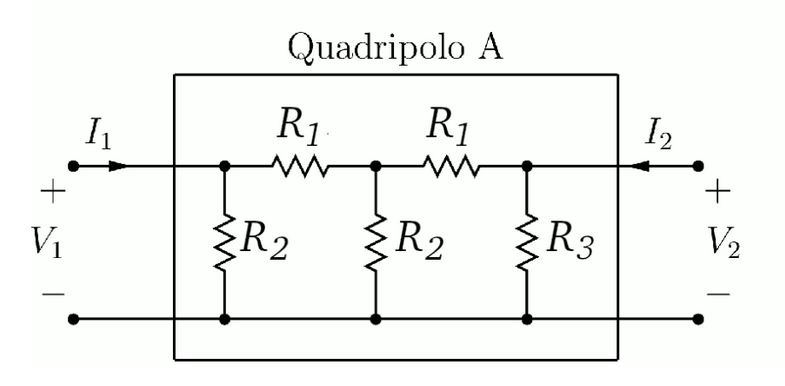
\includegraphics[width=1\columnwidth]{images/quadripoloa.png}
    \caption{Quadripolo "A" puramente resistivo.}
\end{figure}


\begin{figure}[h]
    \centering
    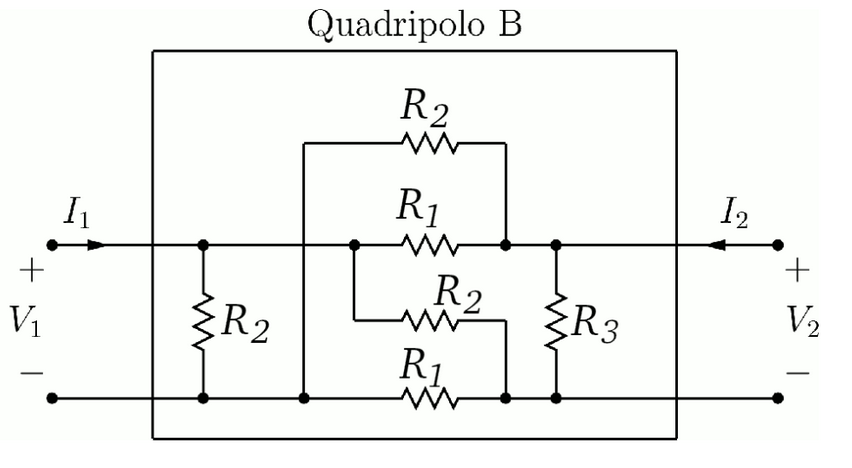
\includegraphics[width=1\columnwidth]{images/quadripolob.png}
    \caption{Quadripolo "B" puramente resistivo.}
\end{figure}

\subsection{Maxima ou Quartus}

Lorem ipsum dolor sit amet, consectetur adipiscing elit. Donec sed turpis condimentum, commodo quam sit amet, dictum ex.

\subsubsection{Quadripolo \emph{A}}

\begin{equation}
    \begin{aligned}
         & {{V_{1}-{\it Va}}\over{R_{1}}}+{{V_{1}}\over{R_{2}}}-I_{1}=0                              \\
         & {{{\it Va}-V_{2}}\over{R_{1}}}+{{{\it Va}-V_{1}}\over{R_{1}}}+{{ {\it Va}}\over{R_{2}}}=0 \\
         & {{V_{2}-{\it Va}}\over{R_{1}}}+{{V_{2}}\over{R_{3}}}-I_{2}=0
    \end{aligned}
\end{equation}

\subsubsection{Quadripolo \emph{B}}

\begin{equation}
    \begin{aligned}
         & {{V_{1}-{\it Vb}}\over{R_{2}}}+{{V_{1}-{\it Va}}\over{R_{1}}}+{{ V_{1}}\over{R_{2}}}-I_{1}=0       \\
         & {{{\it Va}-{\it Vb}}\over{R_{3}}}+{{{\it Va}-V_{1}}\over{R_{1}}}+{{ {\it Va}}\over{R_{2}}}-I_{2}=0 \\
         & {{{\it Vb}-{\it Va}}\over{R_{3}}}+{{{\it Vb}-V_{1}}\over{R_{2}}}+{{ {\it Vb}}\over{R_{1}}}+I_{2}=0 \\
         & V_{2}={\it Va}-{\it Vb}
    \end{aligned}
\end{equation}

\section{Manual de operacao}


Lorem ipsum dolor sit amet, consectetur adipiscing elit. Donec sed turpis condimentum, commodo quam sit amet, dictum ex. Nullam vel odio arcu. Sed non sollicitudin libero, nec tincidunt ex. Aliquam eget nulla quis elit tristique accumsan. Ut a justo eu turpis dictum cursus sed id magna. In quam nunc, venenatis nec rhoncus in, feugiat ac magna. Nullam eu semper nunc.

\section{Resultados experimentais}


Lorem ipsum dolor sit amet, consectetur adipiscing elit. Donec sed turpis condimentum, commodo quam sit amet, dictum ex. Nullam vel odio arcu. Sed non sollicitudin libero, nec tincidunt ex. Aliquam eget nulla quis elit tristique accumsan. Ut a justo eu turpis dictum cursus sed id magna. In quam nunc, venenatis nec rhoncus in, feugiat ac magna. Nullam eu semper nunc.


\section{Discussao dos resultados}

Lorem ipsum dolor sit amet, consectetur adipiscing elit. Donec sed turpis condimentum, commodo quam sit amet, dictum ex. Nullam vel odio arcu. Sed non sollicitudin libero, nec tincidunt ex. Aliquam eget nulla quis elit tristique accumsan. Ut a justo eu turpis dictum cursus sed id magna. In quam nunc, venenatis nec rhoncus in, feugiat ac magna. Nullam eu semper nunc.

\section{Conclusões}

Lorem ipsum dolor sit amet, consectetur adipiscing elit. Donec sed turpis condimentum, commodo quam sit amet, dictum ex. Nullam vel odio arcu. Sed non sollicitudin libero, nec tincidunt ex. Aliquam eget nulla quis elit tristique accumsan. Ut a justo eu turpis dictum cursus sed id magna. In quam nunc, venenatis nec rhoncus in, feugiat ac magna. Nullam eu semper nunc.

\end{document}